%% ******************************************************
%% * This work may be distributed and/or modified under *
%% * the conditions of the LaTeX Project Public License *
%% *     http://www.latex-project.org/lppl.txt          *
%% * either version 1.3c of this license or any later   *
%% * version.                                           *
%% ******************************************************
\PassOptionsToPackage{quiet}{xeCJK}
\PassOptionsToPackage{quiet, no-math}{fontspec}
\documentclass[11pt]{article}
\usepackage{geometry,pdfpages,caption,indentfirst,setspace}
\captionsetup[table]{name={\textsc{Table}},labelsep=period}
\usepackage[level]{datetime}
\usepackage{unicode-math,xeCJK}
\usepackage{authblk,xltxtra}
\usepackage{booktabs,diagbox,ragged2e,tabularx}
\renewcommand\tabularxcolumn[1]{>{\Centering}m{#1}}
\usepackage[toc]{multitoc}
\usepackage[mono=false]{libertine}
% \setstretch{1.25}
\setCJKmainfont{Chiron Sung HK}
[BoldFont=Chiron Sung HK Bold,
  ItalicFont=Kaiti SC]
\usepackage{hyperref,cprotect,xcolor,verbatim,tikz}

\definecolor{pkgcolor}{Hsb}{103,.8,.5}
\definecolor{moducolor}{Hsb}{290,.8,.5}
\definecolor{cmdcolor}{Hsb}{188,.8,.5}
\definecolor{filecolor}{Hsb}{207,.6,.7}
\definecolor{H1}{Hsb}{349,.8,.8} % 海棠紅 (Hangzhou MTR L 1 )
\definecolor{H2}{Hsb}{23, .8,.8} % 丹桂橙 (Hangzhou Metro 2 )
\definecolor{H3}{Hsb}{48, .8,.8} % 柠檬黄 (Hangzhou Metro 3 )
\definecolor{H4}{Hsb}{103,.8,.8} % 香樟绿 (Hangzhou Metro 4 )
\definecolor{H5}{Hsb}{188,.8,.8} % 青藍色 (Hangzhou MTR L 5 )
\definecolor{H6}{Hsb}{207,.8,.8} % 海洋蓝 (Hangzhou Metro 6 )
\definecolor{H7}{Hsb}{290,.8,.8} % 浪漫紫 (Hangzhou Metro 7 )
\hypersetup{colorlinks,urlcolor=H6,linkcolor=H2,filecolor=filecolor,pdfstartview=FitH,pdfview=FitH,pdfcreator=XeTeX output}

\def\pkg#1{\texorpdfstring{\textcolor{pkgcolor}{\textsf{#1}}}{“#1”}}
\def\mode#1{\texorpdfstring{\textcolor{moducolor}{\textsf{#1}}}{“#1”}}
\def\cmd#1{\texorpdfstring{\textcolor{cmdcolor}{\textsf{#1}}}{“#1”}}
\def\datechange#1#2{%
  \noindent{\makebox[\textwidth][r]{\color{H7}\rule{1.15\textwidth}{.4pt}}}
  \noindent\makebox[0pt][r]{\makebox[-3em][r]{\small\textbf{\textcolor{H7}{#1}}}\;\;}{\sffamily Update: \ignorespaces#2}}
\makeatother

\title{\bfseries The \pkg{LiteTable} Template}
\author{Xia Mingyu, \href{https://www.hdu.edu.cn}{Hangzhou Dianzi University}}
\yyyymmdddate
\date{\today}
\affil{\href{mailto:xiamyphys@gmail.com}{\ttfamily xiamyphys@gmail.com}}
\date{\today\quad Version 2.4a\thanks{%
  \url{https://github.com/xiamyphys/litetable}}}
\begin{document}
\maketitle

\vspace{-2em}
\begin{abstract}
This is the document for \pkg{LiteTable} template, which provides a beautiful design of class schedule with colorful course blocks.
\end{abstract}

\tableofcontents

\clearpage

\section{Introduction}

\subsection{The purpose of this template}
This template provides a beautiful design of class schedule with colorful course blocks.

If you meet bugs when using this template, or you have better suggestions or ideas, or you want to participate in the development of the template or other templates by me, welcome to contact via email \href{mailto:xiamyphys@gmail.com}{\ttfamily xiamyphys@gmail.com}.

Also, you can join my \textsf\LaTeX{} Template Discussion \href{https://qm.qq.com/q/OnHzbNvVAG}{QQ Group: 760570712} to communicate with me and get the insider preview edition of the template.

\subsection{Packages required}
This template is based on the template \pkg{standalone}. And it requires \pkg{tikz} package to plot some graphics, \pkg{kvoptions} and \pkg{etoolbox} packages to provide global options, \pkg{expl3} package to support \cmd{timelist} array, \pkg{xeCJK} package to support the \textbf{Chinese, Simplified} language and \pkg{fontawesome5} package to provide a set of beautiful icons.

\subsection{Installing \pkg{LiteTable} and loading it}
For portable version, simply download latest \verb|litetable.cls| file from \href{https://github.com/xiamyphys/LiteTable}{GitHub} or \href{https://ctan.org/pkg/litetable}{CTAN} and save it under your working directory. This way of installation is simple and convenient, but you have to manually update \verb|.cls| now and then.

However, I strongly suggest that you should use terminal/cmd to implement the commands to update all the packages (and install this package) to the latest version or switch to portable version instead
\begin{verbatim}
    sudo tlmgr update --self
    sudo tlmgr update --all
\end{verbatim}

If you are in some areas with awful Internet environment (such as GFW), you can choose proper mirror source or use other means\footnote{Please comply with local network regulations.}. To learn more, please refer to \href{https://tex.stackexchange.com/questions/55437/how-do-i-update-my-tex-distribution}{How do I update my \TeX{} distribution?}

The template provides four options, \mode{style}, \mode{direction} and \mode{font}. Just add the modes of the options you want separately in the square bracket of the command \verb|\documentclass[ ]{litetable}| in your \verb|.tex| file.

\subsection{Compatibility}
The test environments are macOS + MacTeX 2023 / Overleaf and they all work fine for \XeLaTeX{} compiler, Windows, Linux and Unix platforms compatibility unknown.

\section{Global Options of \pkg{LiteTable}}
\begin{verbatim}
  \documentclass[options]{litetable}
\end{verbatim}

\subsection{The \mode{style} option}
This option has two modes, \mode{round} and \mode{sharp}, which can make the course block's corners be round or sharp, and the default mode is sharp.

\subsection{The \mode{direction} option}
This option has two modes, \mode{portrait} and \mode{landscape}, which can make the timetable displayed portrait or horizontally.

\subsection{The \mode{font} option}
This option has two modes, \mode{times} and \mode{libertinus}, which can make the font to be ``Times New Roman'' or ``Libertinus'', and the default mode is ``Times New Roman''.\footnote{Please ensure that your computer has been already installed the font ``Libertinus'' when using this option.}

\section{Commands of \pkg{LiteTable}}

\subsection{The \cmd{makeframe} command}
\begin{verbatim}
  \makeframe{Timetable -- Semester 5}
\end{verbatim}

This command can create an empty class schedule with the title ``Timetable -- Semester 5''.

\subsection{The \cmd{weeklist} command}
\begin{verbatim}
  \weeklist{
    \bfseries\textcolor{W1}{\faIcon{moon}~Monday},
    \bfseries\textcolor{W2}{\faIcon{fire}~Tuesday},
    \bfseries\textcolor{W3}{\faIcon{water}~Wednesday},
    \bfseries\textcolor{W4}{\faIcon{tree}~Thursday},
    \bfseries\textcolor{W5}{\faIcon{coins}~Friday}
  }
\end{verbatim}

This command can add workdays to the top side of the timetable, and you can also adjust the format that you like, such as name, color and even the logo\footnote{Supports by the \pkg{fontawesome5} package.} before it.

The timetable can automatically generate the corresponding number of columns based on the number of workdays you enter. For example, the code above has 5 workdays, a 5-column timetable will be generated.

\subsection{The \cmd{timelist} \cmd{classnum} command}
\begin{verbatim}
  \timelist{
    8:05,8:55,10:00,10:50,11:40,13:30,14:20,15:15,16:05,18:30,19:20,20:10;
    8:50,9:40,10:45,11:35,12:25,14:15,15:05,16:00,16:50,19:15,20:05,20:55
  }

  \classnum{14}
\end{verbatim}

The command \cmd{timelist} can add time to the left side of the timetable, and the first line of the content is the start time of the classes while the second line of the content is the end time of the classes, each time separates with a comma (\verb|,|), the first line and the second line separates with a semicolon (\verb|;|).

The timetable can automatically generate the corresponding number of rows based on the number of time groups you enter. For example, the code above has 12 groups of times, a 12-row timetable will be generated.

The command \cmd{classnum} can directly assign the number of rows on the timetable you want without adding time to the left side of the timetable, and there will only be a series of numbers that \emph{aligned vertically to the center of every line}.

The following table shows the effects brought about by the usage of the two commands.
\begin{table}[!ht]
\centering
\caption{Usage of commands \cmd{timelist} and \cmd{classnum}.}

\begin{tabularx}{\textwidth}{c >{\raggedright\arraybackslash}X >{\raggedright\arraybackslash}X}
  \toprule
  \diagbox{\cmd{classnum}}{\cmd{timelist}} & \multicolumn{1}{c}{To use}          & \multicolumn{1}{c}{Not to use}\\
  \midrule
  To use     &
  The effect is like the description of command \cmd{timelist}\newline But the number of rows will be assigned by \cmd{classnum} &
  The effect is like the description of command \cmd{classnum} before\\
  \midrule
  Not to use &
  The effect is like the description of command \cmd{timelist} before &
  The effect is like the description of command \cmd{timelist} before with \emph{default format of 12 lines}\\
  \bottomrule
\end{tabularx}
\end{table}

\begin{itemize}
  \item Assume that \cmd{timelist} has 12 groups of times, and \cmd{classnum} passed a value of 14, then the left side of the timetable will have only 1 -- 12 rows with time while the last two rows without time the label of them is still upward, not vertically aligned in the center.
  \item Assume that \cmd{timelist} has 14 sets of times, and \cmd{classnum} passes a value of 12, then only 12 rows of timetables will be generated with time on the left side of each row, that is, the last two sets of data in \cmd{timelist} will be invalid.
\end{itemize}

\subsection{The \cmd{weeks} command}
\begin{verbatim}
  \weeks{Week 1 -- 16}
\end{verbatim}

This command can assign the default value of the 7th variable of the command \cmd{course}.

\subsection{The \cmd{course} command}
\begin{verbatim}
  \course[H1]{8}{9}{Group Theory}{Building 6 · 211}{Li Ge}[Week 1 -- 16]
\end{verbatim}

There are 7 variables in this command.
\begin{itemize}
  \item The 1st one is the color of the class that you want, from ``H1'' to ``H9'', it's optional and the default value is ``H1''.
  \item The 2nd and 3rd ones is the starting number and ending number of the class.
  \item The 4th one is the name of the class.
  \item The 5th one is the address of the class.
  \item The 6th one is the name of the teacher(s).
  \item The last one is the start week and end week of the timetable, it's optional and the default value is the value that you've adjusted in the command \cmd{weeks} or it will be ``Week 1 -- 12''.
\end{itemize}

\subsection{The \cmd{newday} command}
This command can switch the current weekday to the next day, then the course will move right one grid.

\subsection{The \cmd{more} command}
\begin{verbatim}
  \more{ · School Start: 04 / 03 / 2024  · Summer Vacation: 05 / 07 / 2024}
\end{verbatim}
This command can add remark at the end of the class schedule.

\subsection{The \cmd{sticker} command}
\begin{verbatim}
  \sticker{favicon}
\end{verbatim}
There will be a sticker on the southeast of the page after you add, otherwise it won't.

\subsection{The \cmd{(re)rotatepage} command}
The \cmd{rotatepage} command can change the direction of the timetable temporarily while the \cmd{rerotatepage} command can restore it.

\section{Known Issue: Resolution exceed}
\begin{verbatim}
  Dimension too large. <recently read> \pgfmath@x
\end{verbatim}

When you choose the \mode{landscape} mode and you've added 7 workdays or more (?although the `above' occasion will not occur), it will return this error.

This is mainly caused by the reason that \emph{\textsf{\TeX} has no built-in floating number representation} (Reference: \cprotect{\href{https://tex.stackexchange.com/a/545416/299948}}{How to solve the error `Dimension too large. <recently read> \verb|\pgfmath@x|' while doing the calculations in the table}).

If one can solve this problem through optimization algorithms or other means, welcome submit your code via GitHub: \url{https://github.com/xiamyphys/litetable}, or contact me via email \href{mail:xiamyphys@gmail.com}{\ttfamily xiamyphys@gmail.com}.

\section{Version History}

The design of this course schedule originated from the student course schedule web page\footnote{Only those studying at or graduated from Hangzhou Dianzi University can have the permission of access.} of the \href{https://www.hduhelp.cn/}{HDUHelp} in \href{https://www.hdu.edu.cn}{Hangzhou Dianzi University}\footnote{https://en.wikipedia.org/wiki/Hangzhou\_Dianzi\_University}. The layout is very beautiful and then I used \LaTeX{} to imitate that style and made a class schedule template to share with everyone.

\textsf{\bfseries Version 1.0} was finished on 1 September, 2023 and released on \href{https://www.latexstudio.net/index/details/index/mid/3625.html}{\LaTeX{} Studio} (Hangzhou) and \href{http://xhslink.com/od7Ycw}{Xiaohongshu}, where won the favor of many people.

\textsf{\bfseries Version 2.0a} was finished developing on 1 November, 2023 and released on \href{https://www.latexstudio.net/index/details/index/mid/3636.html}{\LaTeX{} Studio} (Xiaoshan, Hangzhou) and \href{http://xhslink.com/od7Ycw}{Xiaohongshu}. This version used \verb|.cls| files to make the \verb|main.tex| file more concise. Also, this version has added a global option to choose whether the corners of the ``course Block'' to be round or sharp. And this version support adds multiply class schedules in one \verb|.tex| file.

\textsf{\bfseries Version 2.1a} was finished developing on 5 November, 2023. Supports the libertinus font.

\textsf{\bfseries Version 2.2a} was finished developing on 31 January, 2024. This version fixed the bug of resolution exceeded, changed paper type to US letter and support custom course start time and end time.

\textsf{\bfseries Version 2.3a} was finished developing on 2 February, 2024. This version supports automatically generate the corresponding number of rows based on the number of time groups you enter, and in this version, timetable can be displayed horizontally or portrait as you like.

\textsf{\bfseries Version 2.3b} was finished developing on 3 February, 2024. This version optimized coordinate calculation and improved compilation speed.

\textsf{\bfseries Version 2.4a} was finished developing on 24 February, 2024. Happy Lantern Festival! This version supports custom workday display style, and supports hiding time and only showing course program number vertically aligned.

\clearpage

\datechange{2023/09/01}{Version 2.0a}
\begin{itemize}
    \item Supports the course block's corners be round or sharp.
    \item Supports multiply class schedules in one \verb|.tex| file.
\end{itemize}

\datechange{2023/11/05}{Version 2.1a}
\begin{itemize}
    \item Supports the libertinus font.
\end{itemize}

\datechange{2024/01/31}{Version 2.2a}
\begin{itemize}
    \item Fixed the bug of resolution exceeded.
    \item Changed paper type to US letter.
    \item Support custom course start time and end time.
    \item Support add sticker as you like at the southeast of the page.
    \item Provide simplified Chinese documentation.
\end{itemize}

\datechange{2024/02/02}{Version 2.3a}
\begin{itemize}
  \item Supports automatically generate the corresponding number of rows based on the number of time groups you enter.
  \item Timetable can be displayed portrait or horizontally as you like.
\end{itemize}

\datechange{2024/02/03}{Version 2.3b}
\begin{itemize}
  \item Optimized coordinate calculation and improved compilation speed.
\end{itemize}

\datechange{\today}{Version 2.4a}
\begin{itemize}
  \item Supports custom workday display style.
  \item Supports hiding time and only showing course program number vertically aligned.
  \item Supports setting default first and last week.
\end{itemize}

\appendix

\includepdf[pages={2,4},nup=1x2,pagecommand={
  \tikz[remember picture, overlay]
  \node [rotate=90,below,yshift=-1em] at (current page.west) {\bfseries\LARGE Document Example: \texttt{litetable-demo.tex}};
  }
]{litetable-demo.pdf}
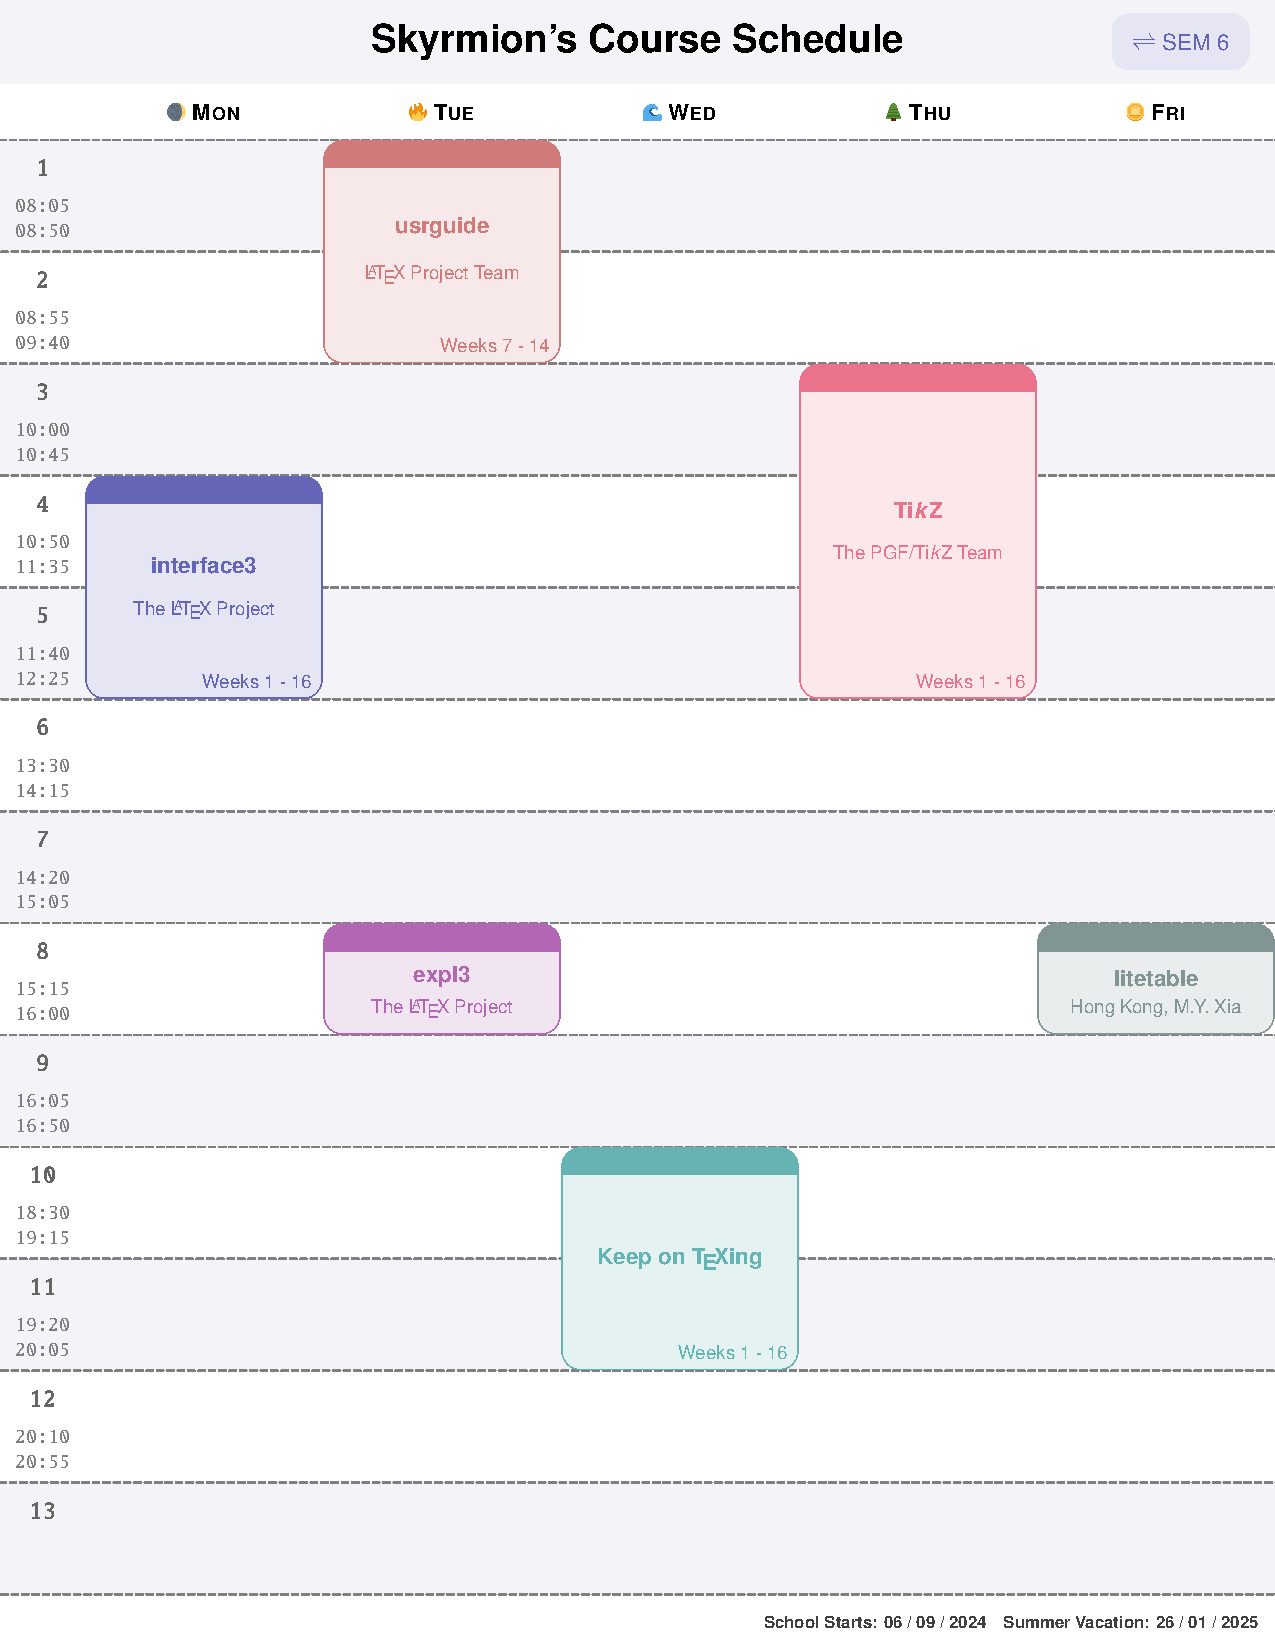
\includepdf[pages={1,3}]{litetable-demo.pdf}

\end{document}